\chapter{演奏音の発音可能な音高範囲の指定}
演奏音の発音可能な音高範囲(以下,音高範囲)を指定する手法について述べる.

\section{実装手法}
RealSenseで扱えるカラー画像の最大サイズは1920$\times$1080である.しかし本研究では主に深度画像を扱うため深度画像の最大サイズ640$\times$480がインタフェースの画面サイズとなる.
本研究のインタフェースは現在発音可能な音を,画面のサイズを音の数で均等に分けて色分けされた領域で表示している.
出力する音の数が多くなるほど一つの音の領域が狭くなり,望む領域に指先を合わせづらくなるため出力できる音高範囲を2オクターブまでとしている.
これによって演奏中に範囲外の音を出力したい場合,出力範囲を変更する必要がある,
しかし,音高範囲の変更を図\ref{img:jesture}のジェスチャーを使って実装する場合,どのジェスチャーも認識精度が悪く演奏中に素早く動かす操作として扱いづらい.そこでジェスチャーに音高範囲の変更を割り当てるのではなく比較的素早く認識する深度を使って演奏モードと音高範囲の変更モードを切り替える方式にした.手をカメラ側に伸ばし音高範囲の変更モードにしたあと画面をスライドさせるような動きをすることで音高範囲が上下にスライドする.音高変更モードに切り替わる深度の範囲(以下,音高変更範囲)はユーザとカメラの距離で変わる.ユーザーの前方の一定範囲を常にtapを認識する範囲とし(以下,tap認識範囲),tap認識範囲のカメラ側の端からカメラまでの範囲を音高変更範囲とした.図\ref{img:range}に概要を示す.

\begin{figure}[t]
	\begin{center}
		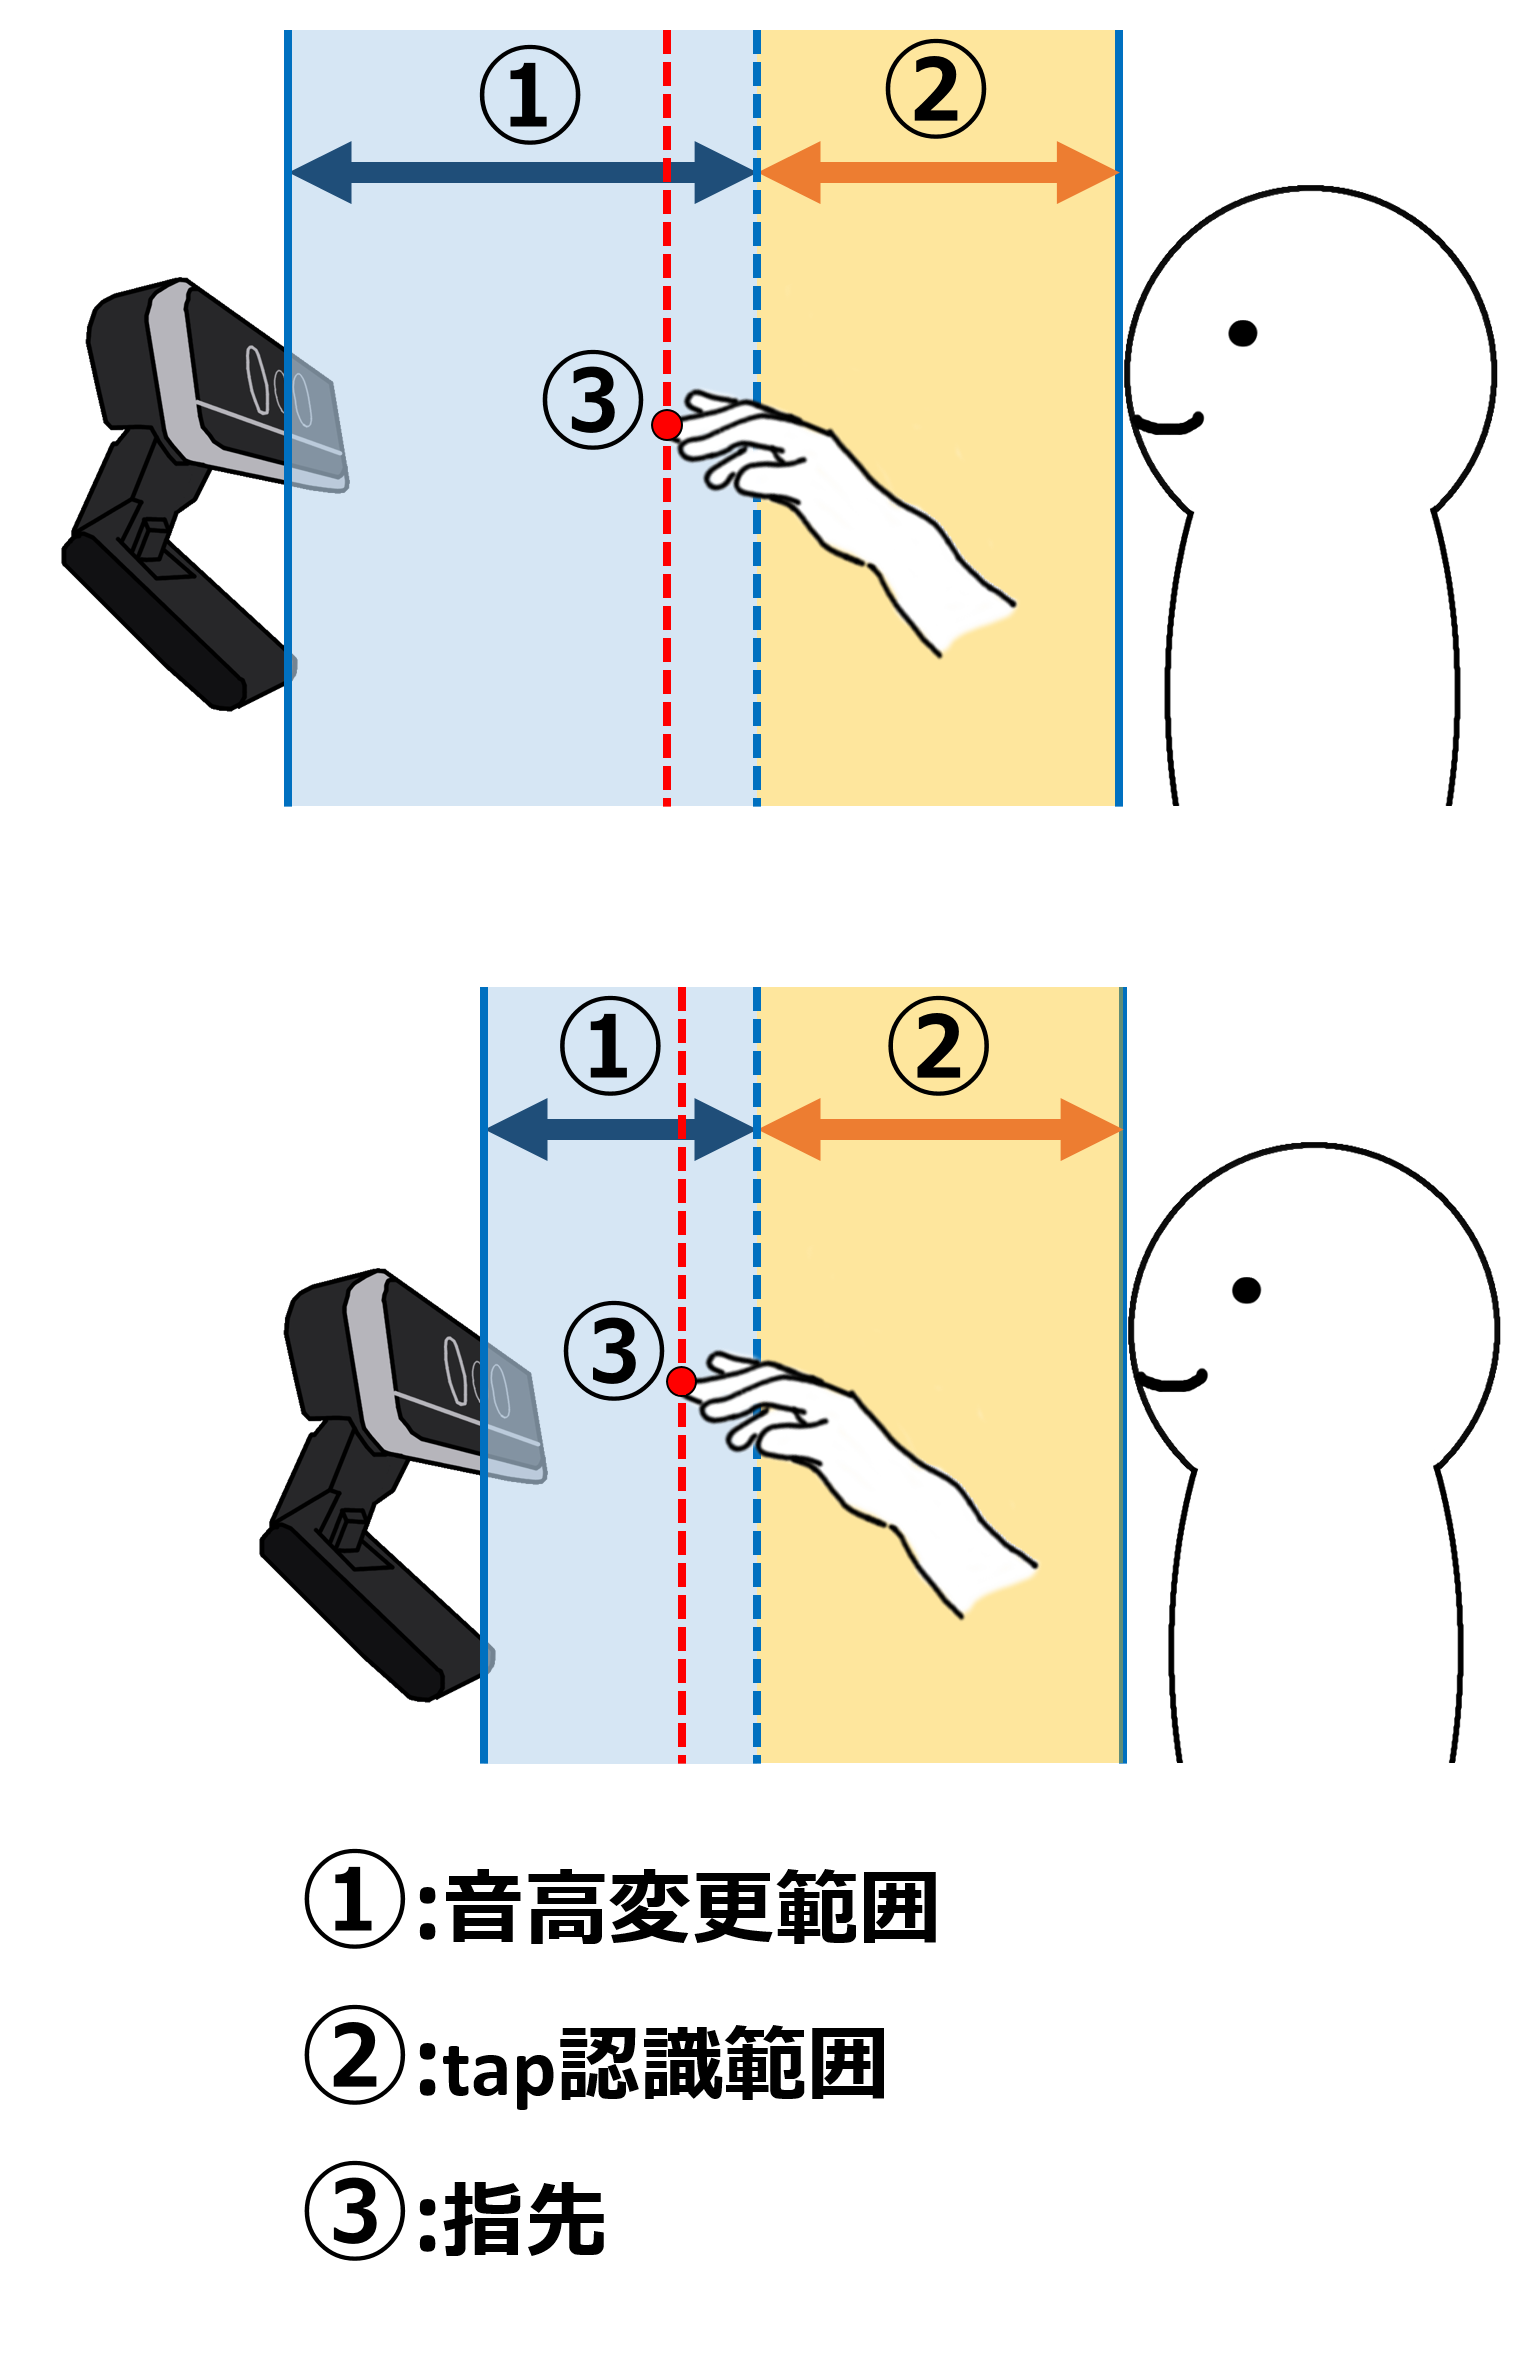
\includegraphics[width=0.9\linewidth]{./pics/04/pitchi_range_change.png}
		\caption{音高変更範囲とtap認識範囲}
		\label{img:range}
	\end{center}
\end{figure}

\section{実行結果と考察}
図\ref{img:red},図\ref{img:blue}に実行結果を示す.音高範囲変更中であることがわかりやすいように指先が音高変更領域に入ったら色のついた円を表示させるようにした.出力範囲は赤,黄,緑,青,紫の順に低くなっていく.この手法によって出力範囲を変更すれば6オクターブ分の範囲の音を出すことができた.これは61鍵(5オクターブ)ピアノの音高範囲より多いのでユーザーが出したい音をカバーできると考えられる.しかし,音高範囲変更中の手は演奏ができないため演奏の自由度が下がるため,なるべく音高変更機能を使わないようにするため,音高範囲の音の数の多さとの一つの音の領域が操作しやすいサイズとなることを両立させた音高範囲の取り方を今後の課題としたい.
\begin{figure}[htbt]
	\begin{center}
		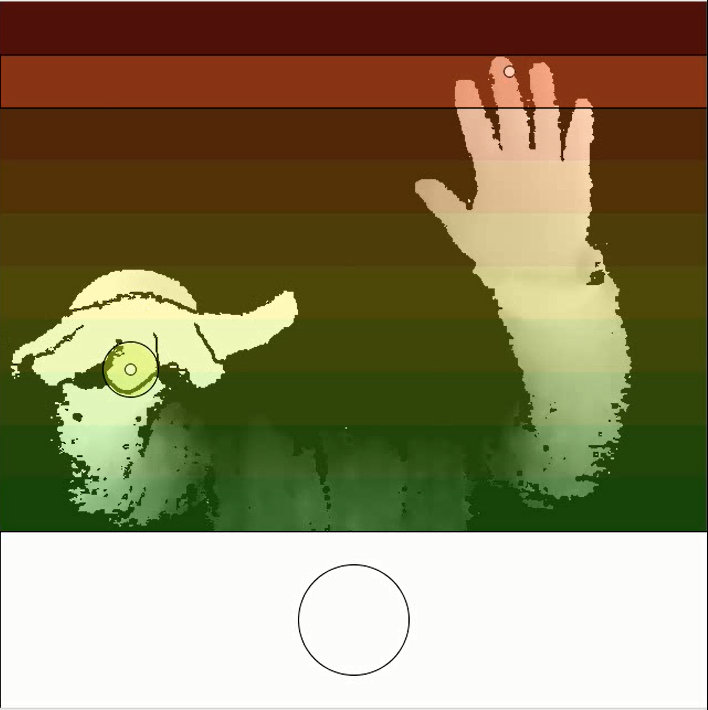
\includegraphics[width=0.5\linewidth]{./pics/04/red.png}
		\caption{出力範囲の変更(高音)}
		\label{img:red} 
	\end{center}
\end{figure}

\begin{figure}[htbt]
	\begin{center}
		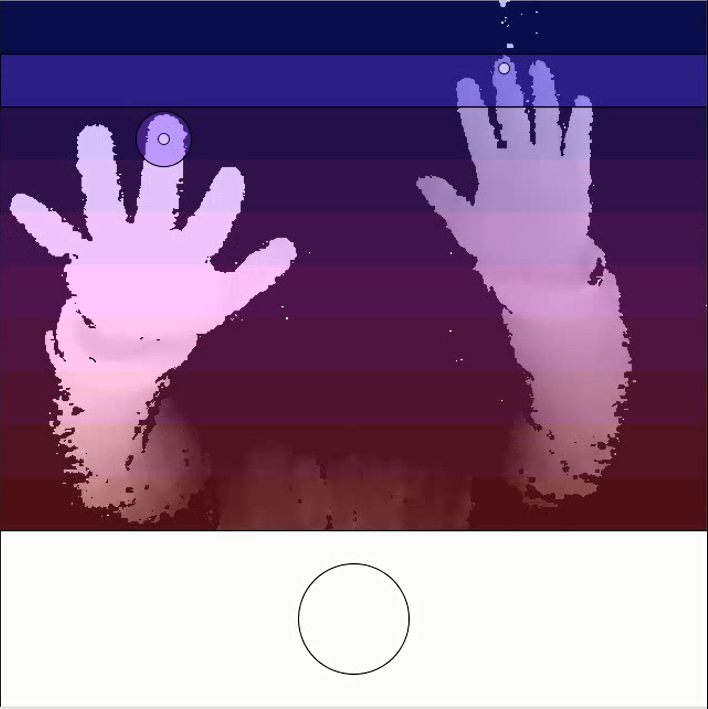
\includegraphics[width=0.5\linewidth]{./pics/04/blue.png}
		\caption{出力範囲の変更(低音)}
		\label{img:blue} 
	\end{center}
\end{figure}